\def\mySecNum{13.2}
\mySection{\mySecNum~Market-maker risk}
%-------------- start slide -------------------------------%{{{ 1
\begin{frame}[fragile,t]
 \begin{itemize}
   \item Market-makers attempt to hedge the risk of their positions.
     \bigskip
   \item Market-makers can control risk by \textcolor{magenta}{Delta-hedging}.
     \bigskip
   \item A hedged position should earn the risk-free rate.
 \end{itemize}
\end{frame}
%-------------- end slide -------------------------------%}}}
%-------------- start slide -------------------------------%{{{ 1
\begin{frame}[fragile,t]
  % \frametitle{Option risk in the absence of hedging}
 \begin{center}
   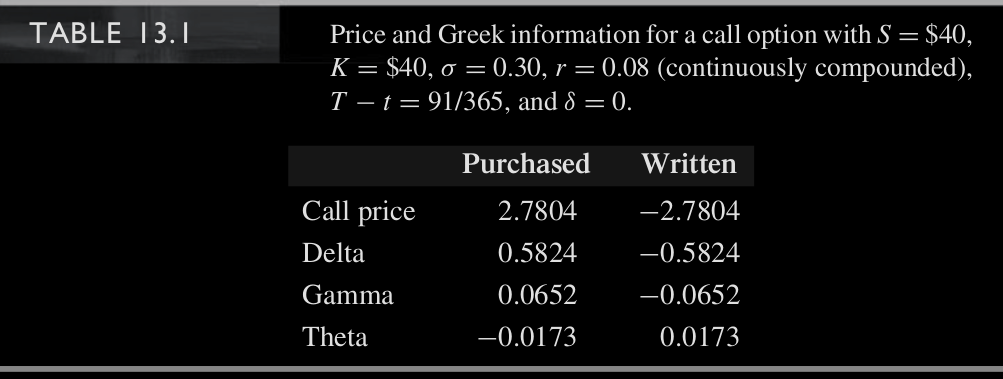
\includegraphics[scale=0.25]{figs/Table_13-1.png}
 \end{center}
\begin{myexample}
  Under setting of the above table,
  \begin{itemize}
    \item compute call price, Delta, Gamma and Theta.
    \item If stock price increases to $S=40.75$,
    \item[] find the exact gain/loss of the market-maker.
    \item[] find the approximate gain/loss of the market-maker via $\Delta$.
    \item If stock price decreases to $S=39.25$,
    \item[] find the exact gain/loss of the market-maker.
    \item[] find the approximate gain/loss of the market-maker via $\Delta$.
  \end{itemize}
  (Assume we liquidate the position at the same day)
\end{myexample}
\vfill
\begin{mysol}
   Try \textcolor{gray}{codes/Section\_13-2.nb}\myEnd
\end{mysol}
\end{frame}
%-------------- end slide -------------------------------%}}}
%-------------- start slide -------------------------------%{{{ 1
\begin{frame}[fragile,t]
  \centering

\end{frame}
%-------------- end slide -------------------------------%}}}
